\documentclass[12pt]{article}
\usepackage[margin=1in]{geometry}
\usepackage{amsmath}
\usepackage{tikz}
\usepackage{pgfplots}
\usepackage{eso-pic}
\pgfplotsset{compat=1.18}

\AddToShipoutPictureBG{%
  \begin{tikzpicture}[remember picture,overlay]
    \foreach \y in {0,1,...,27} {
      \draw[gray!20, very thin] 
        ([yshift=-\y cm]current page.north west) -- 
        ([yshift=-\y cm]current page.north east);
    }
  \end{tikzpicture}
}

\setlength{\parindent}{0pt}
\setlength{\parskip}{8pt}

\title{Week 7: Systems Applications \& Inequalities}
\author{
	Student: SA\\
	Tutor: Rachel Eglash}
\date{October 29, 2025}

\begin{document}
	
	\maketitle

	\section*{Session 7 Quiz}
        
        \subsection*{7.1: Systems Word Problems Mixture, Motion, Break-Even}

	    \subsection*{7.2: Systems of Inequalities}
        
        \subsection*{7.3: Linear Modeling \& Fit-by-Eye}
	    
            \newpage
	
	\section*{Session 7 Quiz: Systems Applications \& Inequalities}

        \vspace{1cm}
	
	    \subsection*{Quick Reference: Key Formulas}
	
	        \subsubsection*{Mixture Problems}
		    	(concentration$_1$)(volume$_1$) + (concentration$_2$)(volume$_2$) = (concentration$_{\text{final}}$)(volume$_{\text{final}}$)
	
	        \subsubsection*{Motion Problems}
			    distance = rate $\times$ time \quad ($d = rt$)
	
	        \subsubsection*{Break-Even Problems}
	    		Total Cost = Total Revenue
	
            \subsubsection*{Residuals}
		    	Residual = Actual value - Predicted value

            \newpage
	
        \subsection*{7.1 Problem 1: Mixture Problem}
            
            A chemist needs to prepare 100 mL of a 16 mg/mL saline solution.\\\\
            She has solution "A", which is a 10 mg/mL solution.\\\\
            She has solution "B", which is a 20 mg/mL solution.\\\\
            How much of each should she mix?

            \newpage
        
        \subsection*{7.1 Problem 2: Motion Problem}

            Two cars leave the same parking lot at the same time.\\\\
            They travel in opposite directions.\\\\
            Car A travels at 50 mph.\\\\
            Car B travels at 70 mph.\\\\
            After how many hours will they be 240 miles apart?
        
            \newpage
        
        \subsection*{7.1 Problem 3: Break-Even Problem}
        
            A sandwich shop makes sandwiches.\\\\	
            The costs include a fixed cost of \$6000 per month,\\\\
            plus a cost of \$2 per sandwich to produce.\\\\
            The revenue from each sandwich is \$8.\\\\
            How many sandwiches must be sold to break even?

            \newpage
        
    	\subsection*{7.2 Problem 4: Basic System}
		
            \textbf{Graph the system of inequalities:}\\\\
			$y \geq 2x - 3$\\\\
			$y < -3x + 7$

			\vspace{1cm}

			\begin{center}
			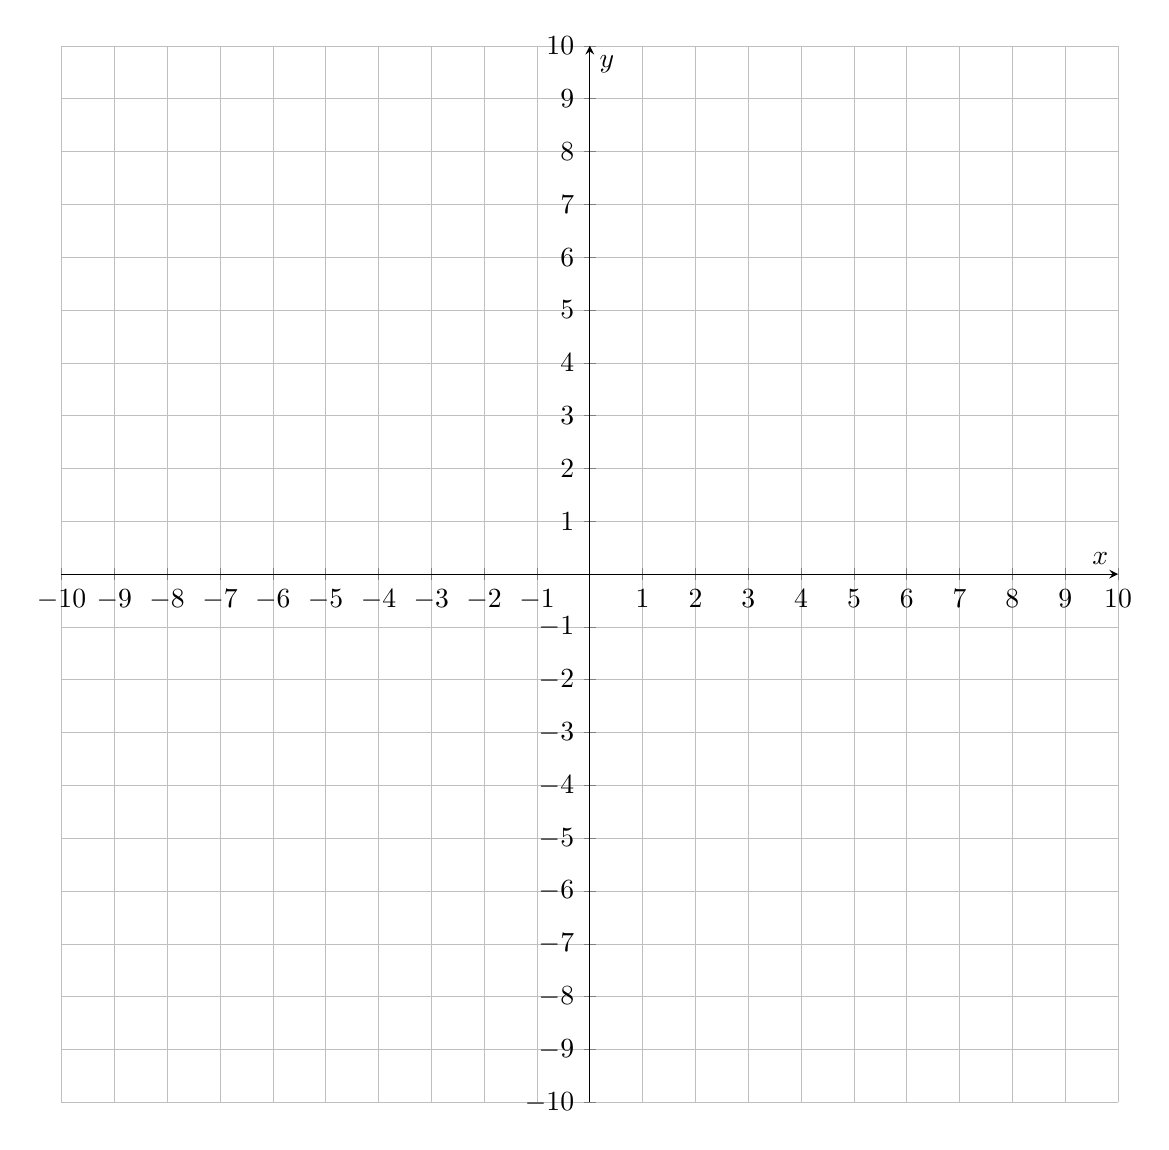
\begin{tikzpicture}
				\begin{axis}[
                    axis background/.style={fill=white},
					xlabel={$x$},
					ylabel={$y$},
					xmin=-10, xmax=10,
					ymin=-10, ymax=10,
					xtick={-10,-9,-8,-7,-6,-5,-4,-3,-2,-1,0,1,2,3,4,5,6,7,8,9,10},
					ytick={-10,-9,-8,-7,-6,-5,-4,-3,-2,-1,0,1,2,3,4,5,6,7,8,9,10},
					grid=both,
					grid style={line width=.1pt, draw=gray!30},
					major grid style={line width=.2pt,draw=gray!50},
					width=15cm,
					height=15cm,
					axis lines=middle,
					enlargelimits=false,
				]
				\end{axis}
			\end{tikzpicture}
			\end{center}
	
	        \newpage
	
	    \subsection*{7.2 Problem 5: Bounded Inequalities}
		
		    \textbf{Graph the system of compound inequalities:}\\\\
			$2 < x < 7$\\\\
			$-1 \leq y \leq 3$

	        \vspace{1cm}

			\begin{center}
			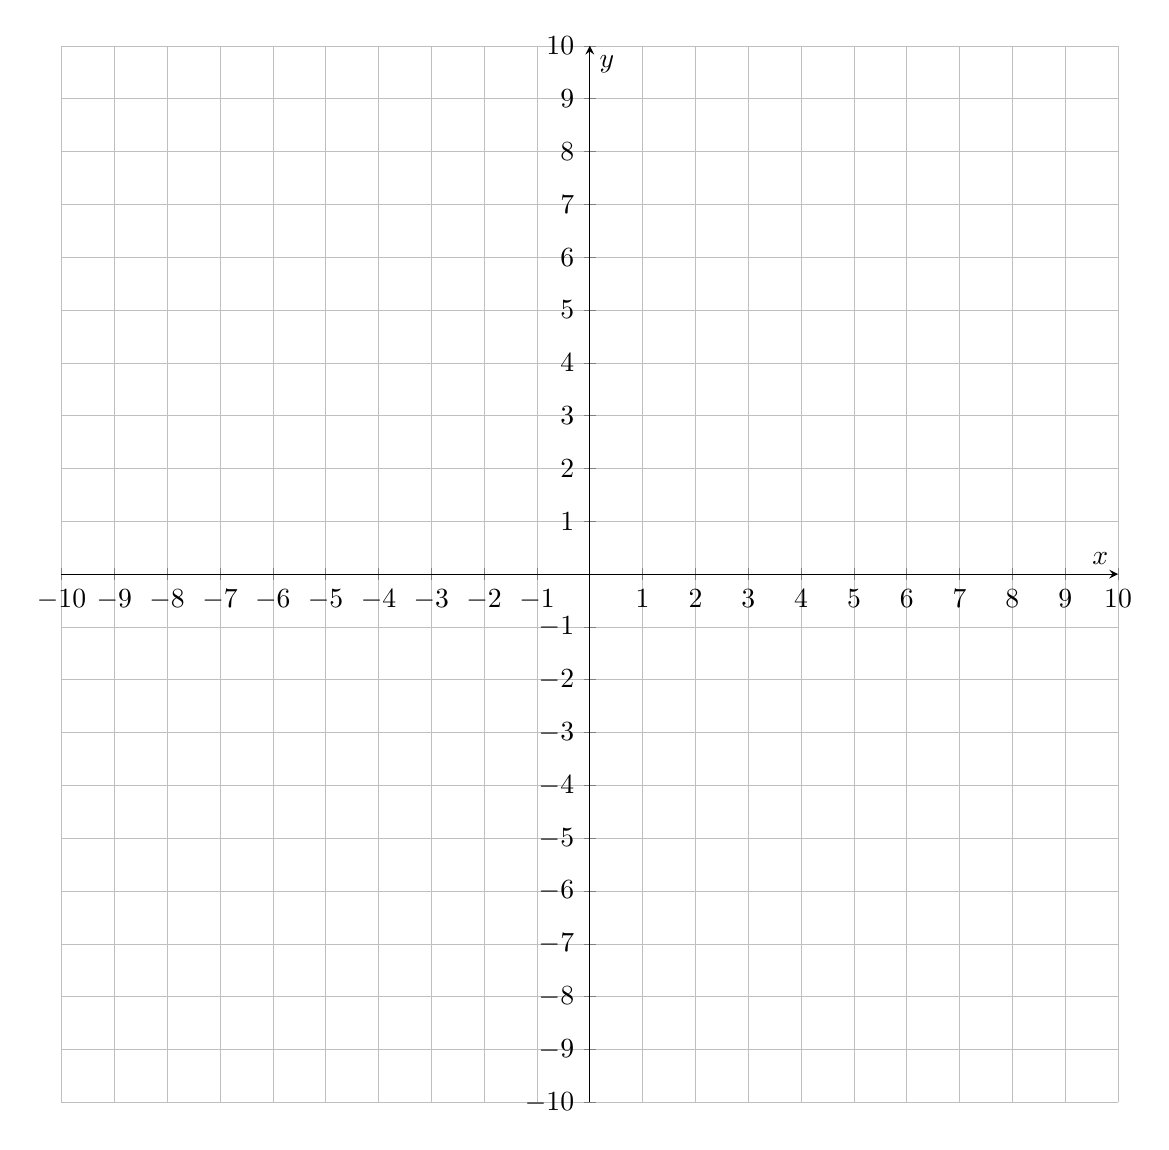
\begin{tikzpicture}
				\begin{axis}[
                    axis background/.style={fill=white},
					xlabel={$x$},
					ylabel={$y$},
					xmin=-10, xmax=10,
					ymin=-10, ymax=10,
					xtick={-10,-9,-8,-7,-6,-5,-4,-3,-2,-1,0,1,2,3,4,5,6,7,8,9,10},
					ytick={-10,-9,-8,-7,-6,-5,-4,-3,-2,-1,0,1,2,3,4,5,6,7,8,9,10},
					grid=both,
					grid style={line width=.1pt, draw=gray!30},
					major grid style={line width=.2pt,draw=gray!50},
					width=15cm,
					height=15cm,
					axis lines=middle,
					enlargelimits=false,
				]
				\end{axis}
			\end{tikzpicture}
			\end{center}
	
	        \newpage
	
	    \subsection*{7.2 Problem 6: Inequality Application}
		
            A bakery makes cookies and brownies.\\\\
		    Each cookie batch requires 2 hours of labor.\\\\
		    Each brownie batch requires 3 hours of labor.\\\\
		    The bakery has \underline{at most} 30 hours of labor per day.\\\\
		    They must make \underline{at least} 2 cookie batches per day.\\\\
		    Write and graph a system of inequalities.

			\vspace{1cm}

			\begin{center}
			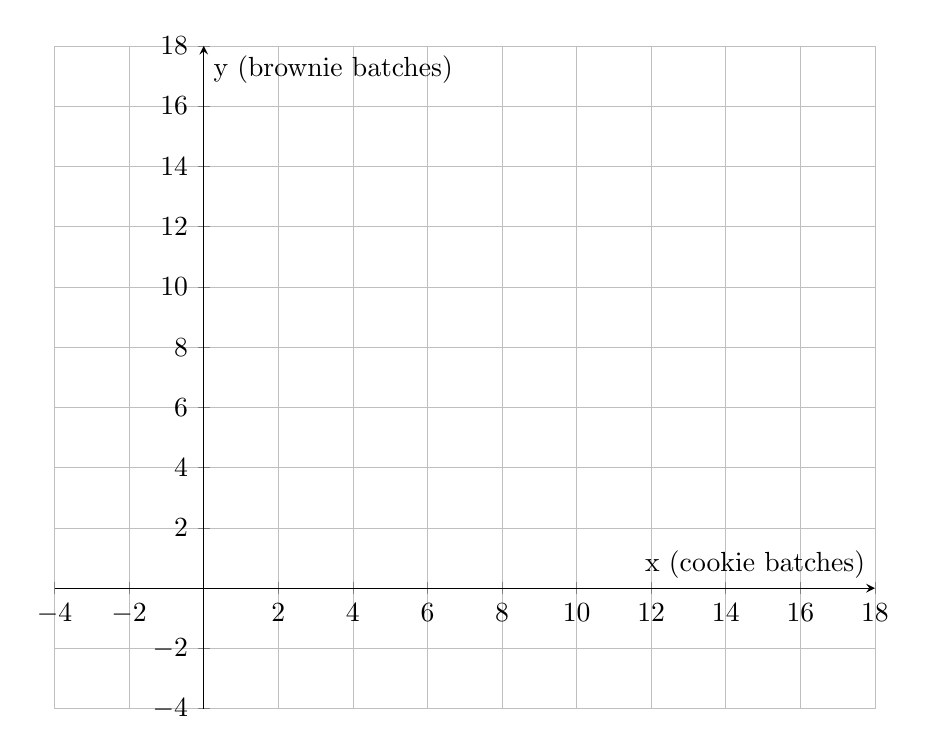
\begin{tikzpicture}
				\begin{axis}[
                    axis background/.style={fill=white},
					xlabel={x (cookie batches)},
					ylabel={y (brownie batches)},
					xmin=-4, xmax=18,
					ymin=-4, ymax=18,
					xtick={-4,-2,0,2,4,6,8,10,12,14,16,18},
					ytick={-4,-2,0,2,4,6,8,10,12,14,16,18},
					grid=both,
					grid style={line width=.1pt, draw=gray!30},
					major grid style={line width=.2pt,draw=gray!50},
					width=12cm,
					height=10cm,
					axis lines=middle,
					enlargelimits=false,
				]
				\end{axis}
			\end{tikzpicture}
			\end{center}
	
	        \newpage
	
		\subsection*{7.3 Problem 7: Study Time and Quiz Score}

			A teacher tracks student study time and quiz scores.

			\begin{center}
				\begin{tabular}{|c|c|}
					\hline
					Study Time (hours) & Quiz Score (\%) \\
					\hline
					1 & 60 \\
					2 & 68 \\
					3 & 76 \\
					4 & 83 \\
					5 & 90 \\
					\hline
				\end{tabular}
			\end{center}

			\subsubsection*{Part A}
			
				Plot the points.

				\begin{center}
				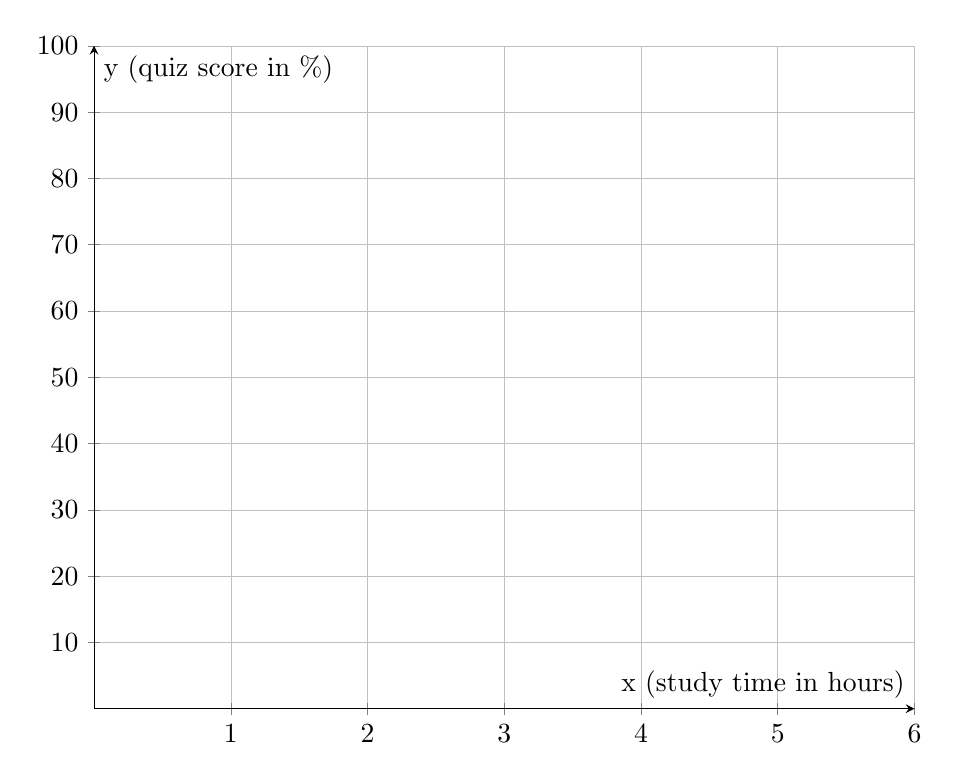
\begin{tikzpicture}
					\begin{axis}[
                        axis background/.style={fill=white},
						xlabel={x (study time in hours)},
						ylabel={y (quiz score in \%)},
						xmin=0, xmax=6,
						ymin=0, ymax=100,
						xtick={0,1,2,3,4,5,6},
						ytick={0,10,20,30,40,50,60,70,80,90,100},
						grid=both,
						grid style={line width=.1pt, draw=gray!30},
						major grid style={line width=.2pt,draw=gray!50},
						width=12cm,
						height=10cm,
						axis lines=middle,
						enlargelimits=false,
					]
					\end{axis}
				\end{tikzpicture}
				\end{center}

                \newpage

			\subsubsection*{Part B}

				Find the equation of the line of best fit.

				\vspace{6cm}

			\subsubsection*{Part C}
				
				Calculate the residual for $x = 3$ hours of study time:

				\vspace{5cm}

			\subsubsection*{Part D}
				
				Use your model to predict the quiz score for someone who studies 8 hours.\\\\
                Is this prediction reasonable? Why or why not?
	
\end{document}